\chapter{سخت‌افزار و الکترونیک}



\section{هسته‌ی پردازشی}

\begin{figure}[h]
	\centering
	\begin{subfigure}{0.45\textwidth}
		\centering
		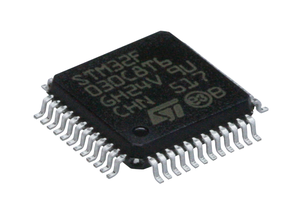
\includegraphics[width=\linewidth]{stm32f030}
		\caption{جداگانه}
		\label{fig:stm32_image}
	\end{subfigure}
	\begin{subfigure}{0.45\textwidth}
		\centering
		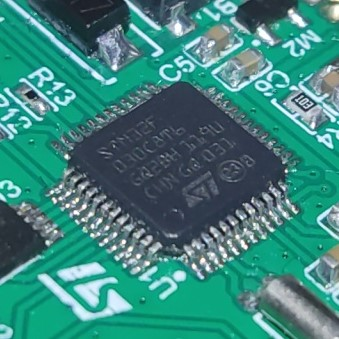
\includegraphics[width=\linewidth]{stm32f030_real}
		\caption{مونتاژ شده روی برد پروژه}
		\label{fig:stm32_real}
	\end{subfigure}
	\caption{تصاویری از پردازنده \lr{STM32F030}}
	\label{fig:stm32}
\end{figure}

\begin{figure}
	\centering
	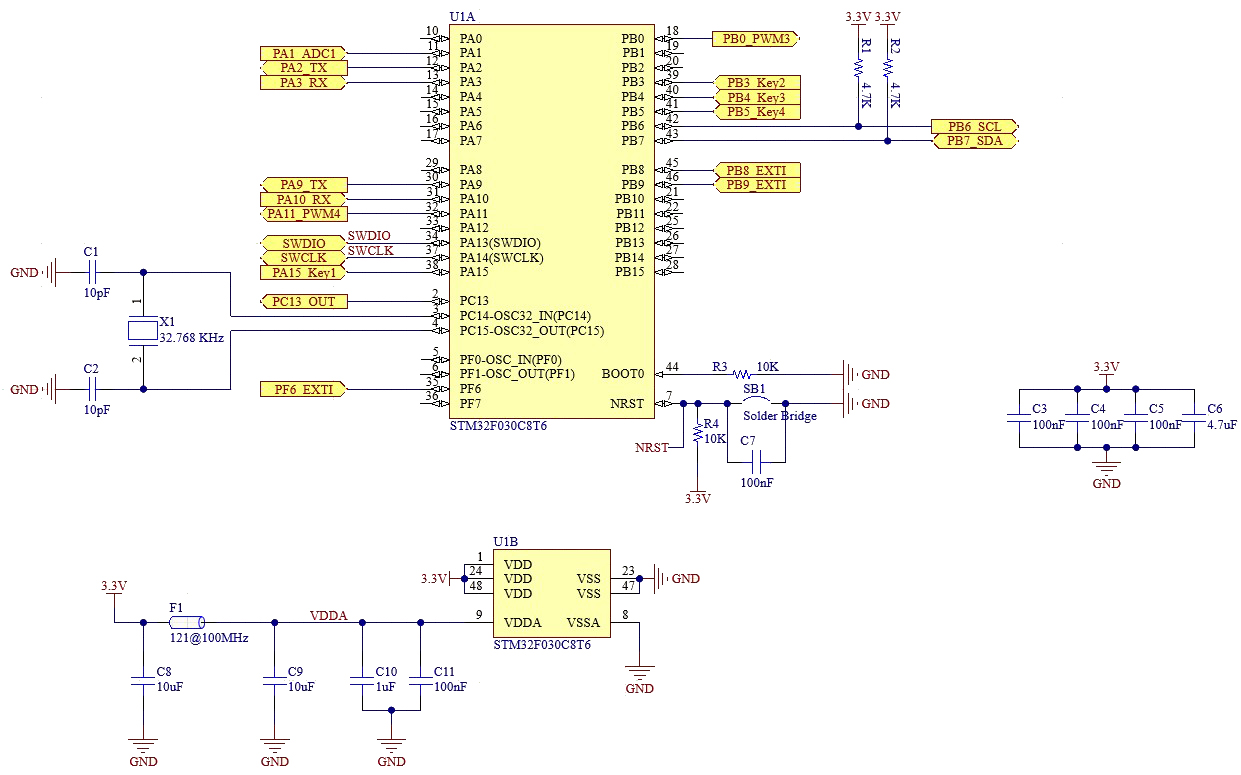
\includegraphics[width=\textwidth]{sch_mcu}
	\caption{شماتیک مربوط به بخش ریزپردازنده}
	\label{fig:ecma1}
\end{figure}


اگر تاریخچه بوجود آمدن اکماسکریپت \ref{fig:stm32_real} و جاواسکریپت (\cref{fig:ecma1}) را بررسی کنیم متوجه تقدم و تاخر زمانی عجیبی خواهیم شد. جاواسکریپت در سال 1996 پدید آمده، و در سال 1997 برای استانداردسازی به اکما ارسال شده است و پس از آن استاندارد اکماسکریپت پدید آمده! بنابراین می‌توان گفت این دو مثل مرغ و تخم‌مرغ بوده‌اند و با اینکه جاواسکریپت منطبق بر استاندارد اکما پیش می‌رود و نسبت به آن موخر است، اما در اولین انتشار، خودش باعث بوجود آمدن استاندارد اکما شده است!

کاربرد اصلی و اولیه جاواسکریپت، ایجاد عملکرد\footnote{\lr{Functionality}} در صفحات وب بود. درواقع، سومین تکنولوژی که توسط کنسرسیوم شبکه جهانی وب\footnote{\lr{W3C}} برای استفاده همگانی توسط تمامی مروگرهای پشتیبانی‌کننده از استانداردهای وب استفاده شد، در کنار زبان‌های ایجادکننده ظاهر و قالب (شامل اچ‌تی‌ام‌ال\footnote{\lr{HTML}} و سی‌اس‌اس\footnote{\lr{CSS}}) استاندارد دام\footnote{\lr{DOM (Document Object Model)}} بود و در عمل جاواسکریپت برای کنترل و ارائه دام توسط دو شرکت نت‌اسکیپ\footnote{\lr{Netscape}} و سان میکروسیستمز\footnote{\lr{Sun Microsystems}} طراحی شد؛ بعدها با الحاق به استاندارد اکماسکریپت و پیروی از آن، به جاواسکریپت امروزی تبدیل شد که قابلیت استفاده گسترده در مرورگرهای وب و خارج از آن‌ها را دارد\cite{ecma}.


%\subsection{گوگل وی8}


موتور جاواسکریپت گوگل وی8 (\cref{fig:v8})، یک موتور جاواسکریپت متن‌باز\footnote{\lr{Opensource}} است که توسط گوگل با زبان سی‌پلاس‌پلاس\footnote{\lr{C++}} توسعه پیدا کرده و مرورگر معروف گوگل (گوگل کروم\footnote{\lr{Google Chrome}}) از آن استفاده می‌کند\cite{wiki:v8}.

\newpage

وی8 با ترجمه جاواسکریپت به زبان‌های بومی و محلی ماشین هدف، باعث افزایش کارایی می‌شود. درواقع یکی از تفاوت‌های اجرای جاواسکریپت با زبانی مثل جاوا\footnote{\lr{Java}} در همین است. در فرآیند ترجمه زبان جاوا، خروجی تولید شده نوعی بایت‌کد\footnote{\lr{Bytecode}} است که برای ماشین هدف قابل فهم نخواهد بود و ماشین مجازی جاوا\footnote{\lr{JVM (Java Virtual Machine)}} باید آن را تفسیر و اجرا کند. اما وی8 با ترجمه مستقیم جاواسکریپت به زبان بومی ماشین هدف، مرحله تفسیر و اجرای بایت‌کدهای واسط را حذف کرده و کارآیی را به مقدار قابل توجهی نسبت به بقیه زبان‌های تفسیری (مانند جاوا و پایتون\footnote{\lr{Python}}) افزایش می‌دهد\cite{wiki:v8}.

وی8 بهینه‌سازی‌های جانبی دیگری نیز روی کد جاواسکریپت ورودی انجام می‌دهد، از جمله استفاده از نهانگاه درون‌برنامه‌ای\footnote{\lr{Inline caching}}. بنابراین در کل، جاواسکریپت یکی از زبان‌هایی است که با اینکه همیشه ترجمه نمی‌شود، اما سرعت و عملکرد اجرایی آن با زبان‌های ترجمه شدنی قابل رقابت و مقایسه است\cite{wiki:v8}.

\begin{figure}[H]
	\centering
	
\includegraphics[scale=.3]{v8}
	\caption{لوگوی وی8}
	\label{fig:v8}
\end{figure}

همانطور که پیش‌تر گفته شد، از این موتور جاواسکریپت در چارچوب نودجی‌اس استفاده شده است. البته این موتور تنها موتور جاواسکریپت موجود نیست. برای مثال مرورگر معروف موزیلا فایرفاکس\footnote{\lr{Mozilla Firefox}} از موتور جاواسکریپت اسپایدر مانکی\footnote{\lr{SpiderMonkey}} استفاده می‌کند. همچنین جلوتر در همین سند خواهیم دید که ری‌اکت نیتیو برای اجرای بهتر و سریعتر روی گوشی‌های هوشمند می‌تواند از موتور هرمس\footnote{\lr{Hermes}} (\cref{fig:hermes}) استفاده کند\cite{v8}.

\begin{figure}[H]
	\centering
	
\includegraphics[scale=.3]{hermes}
	
\includegraphics[scale=.1]{spidermonkey}
	\caption{لوگوی هِرمِس و اسپایدر مانکی}
	\label{fig:hermes}
\end{figure}


%\subsection{اجرا، خارج از مرورگر وب}

با توجه به مطالبی که گفته شد،‌ جاواسکریپت در ابتدا فقط برای اجرا بر روی مرورگرهای وب بوجود آمده بود؛ اما بعدها با افزایش قدرت و توسعه کتابخانه‌ها و جامعه کاربری آن، نیاز به اجرای خارج از مرورگر وب برای جاواسکریپت ایجاد شد. در اینجا بود که چارچوب‌هایی نظیر نودجی‌اس بوجود آمدند. درواقع یک چارچوب جاواسکریپت، با ایجاد یک محیط اجرایی\footnote{\lr{Runtime environment}} مناسب در خارج از مرورگر وب، زمینه را برای اجرای کد توسط یک موتور جاواسکریپت (مثلا وی8) فراهم می‌کند\cite{v8}.

\begin{figure}[H]
	\centering
	
\includegraphics[scale=.3]{nodejs}
	\caption{لوگوی نودجی‌اس}
	\label{fig:nodejs}
\end{figure}

در واقع درون جاواسکریپت، اشیائی وجود دارند که به آن‌ها اشیاء میزبان\footnote{\lr{Host objects}} گفته می‌شود. برای مثال، شئ سند\footnote{\lr{document}} درون کد جاواسکریپت اجرایی در یک مرورگر تعریف شده است. اما این شئ میزبان در نودجی‌اس وجود نخواهد داشت. بنابراین جایگزین کردن اشیاء میزبان دیگر مانند اشیاء دسترسی به نظام فایل‌ها\footnote{\lr{Filesystem}}، فرآیندها\footnote{\lr{Processes}} و درخواست‌های تحت شبکه\footnote{\lr{Network requests}} با این شئ از وظایف یک چارچوب جاواسکریپت مانند نودجی‌اس (\cref{fig:nodejs}) است\cite{wiki:nodejs}.

چارچوب‌های معروف دیگری نیز برای جاواسکریپت بوجود آمده‌اند، مانند چارچوب دنو\footnote{\lr{Deno}} (\cref{fig:deno}) که توسط همان سازنده اصلی نودجی‌اس بوجود آمده و درون خود از همان موتور وی8 استفاده می‌کند؛ با این تفاوت که اینبار بجای زبان سی‌پلاس‌پلاس، با زبان راست\footnote{\lr{Rust}} پیاده‌سازی شده است (که طبق آمار می‌تواند از سی‌پلاس‌پلاس سریع‌تر باشد). همچنین ویژگی‌های امنیتی بیشتری نیز به آن به نسبت نودجی‌اس اضافه شده است\cite{wiki:deno}.

\begin{figure}[H]
	\centering
	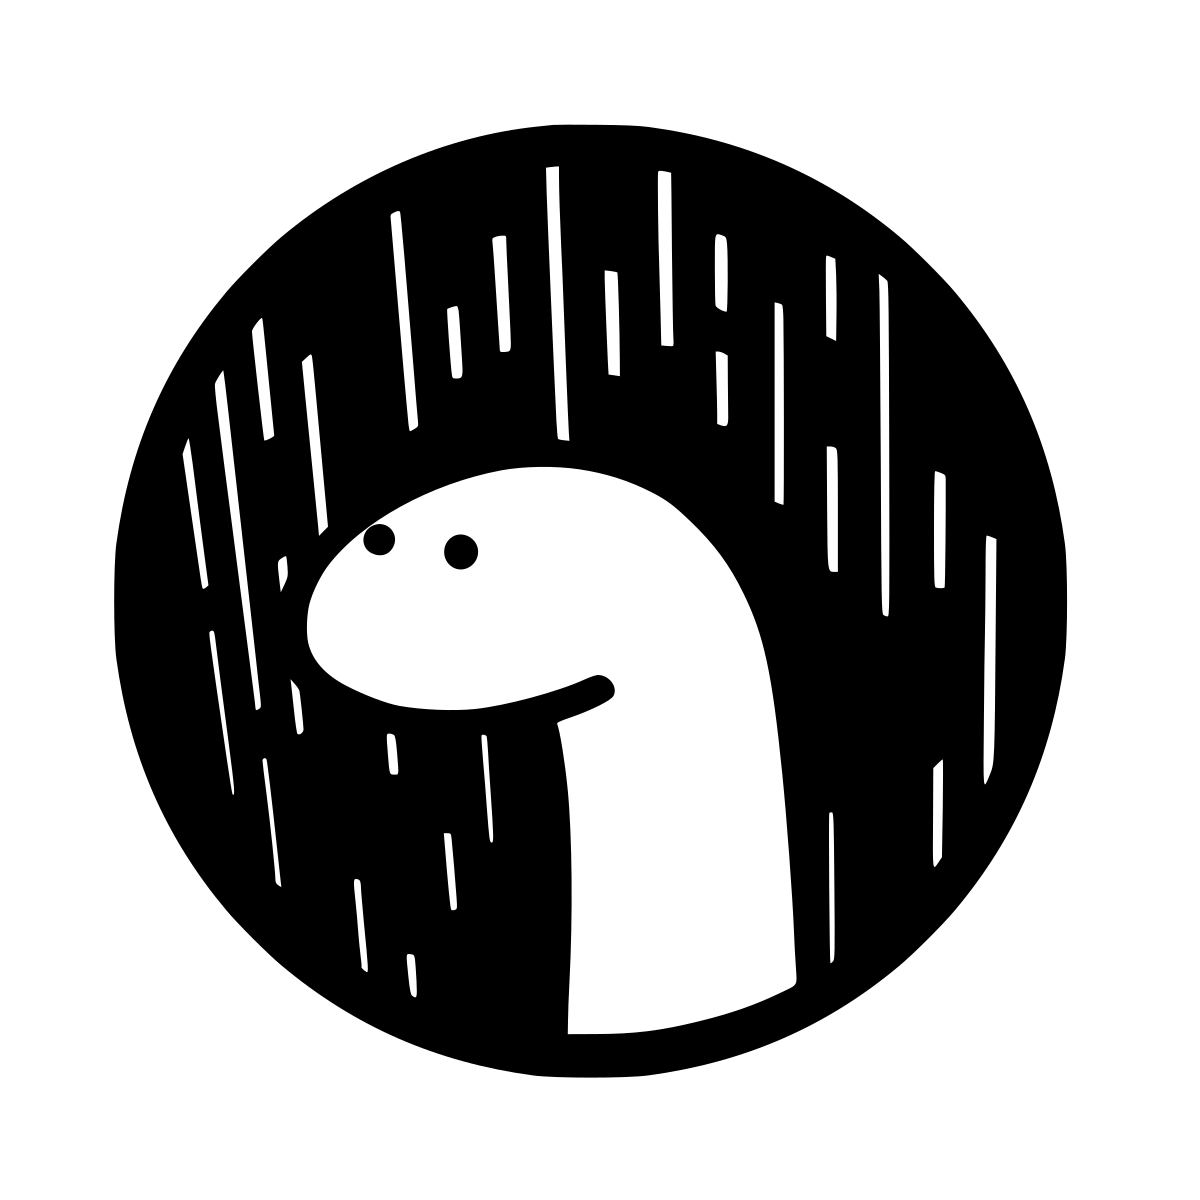
\includegraphics[scale=.3]{deno}
	\caption{لوگوی دِنو}
	\label{fig:deno}
\end{figure}


%\subsection{اکسپرس}

برای استفاده از نودجی‌اس جهت اجرای سرویس‌دهنده‌ی وب، از کتابخانه‌های زیادی می‌توان استفاده کرد. معروف‌ترین کتابخانه موجود برای نودجی‌اس، اکسپرس\footnote{\lr{ٍExpress}} است. کتابخانه‌های دیگری مثل هَپی و کوآ نیز وجود دارند که به ترتیب استفاده کمتری نسبت به اکسپرس در بین جامعه کاربران نودجی‌اس دارند\cite{wiki:express}.

%\subsection{تایپ‌اسکریپت}

زبان جاواسکریپت از نظام نوع‌دهی\footnote{\lr{Type system}} ایستا\footnote{\lr{Static}}یی برای متغیرها پیروی نمی‌کند و اکثر تایپ‌ها در زمان اجرا مشخص می‌شوند. این موضوع برای پیاده‌سازی پروژه‌های بزرگ و منسجم می‌تواند بسیار مشکل‌ساز باشد. به همین‌منظور، زبان‌های زیادی بوجود آمده‌اند که عملا ویژگی‌های جاواسکریپت را به ارث برده‌اند، اما نظام نوع‌دهی ایستا را نیز به آن اضافه کرده‌اند\cite{wiki:ts}.

شرکت مایکروسافت در سال 2012، اولین نسخه مترجم زبان تایپ‌اسکریپت (\cref{fig:ts}) را منتشر کرد. این زبان یک ابرمجموعه از تعریف زبان جاواسکریپت است؛ به این معنا که کدهای جاواسکریپت بدون هیچ تغییری در زبان تایپ‌اسکریپت معتبر هستند، اما می‌توان برای متغیرهای موجود در آن‌ها نوع‌دهی ایستا و سخت‌گیرانه انجام داد. تایپ‌اسکریپت از نوع‌دهی‌های بسیار به‌روز و پیشرفته‌ای برای مدیریت انواع حالت‌ها و شرایط پیچیده استفاده می‌کند که می‌تواند کیفیت و خوانایی کدهای تولید شده را بشدت افزایش داده و در عین حال، نگهداری از آن‌ها را بسیار ساده‌تر کند\cite{wiki:ts}.

\begin{figure}[H]
	\centering
	
\includegraphics[scale=.2]{ts}
	\caption{لوگوی تایپ‌اسکریپت}
	\label{fig:ts}
\end{figure}


نکته بسیار مهم در مورد تایپ‌اسکریپت این است که خروجی تولیدشده توسط مترجم تایپ‌اسکریپت، کد جاواسکریپت معادل آن است! بنابراین تایپ‌اسکریپت می‌تواند بصورت یک لایه اضافه بر روی جاواسکریپت سوار شود و پس از انجام ترجمه، موتورهای جاواسکریپت ادامه کار را بدست بگیرند. یکی از مزایای این نوع ترجمه، عدم تاثیر حجم اضافه شده به کد در اثر استفاده از نظام نوع‌دهی بر روی کارایی و سرعت اجرای کد است.

تایپ‌اسکریپت تنها راهکار بوجود آمده برای تکمیل زبان جاواسکریپت نیست؛ بلکه خروجی مترجم‌های دیگری مثل بیبل\footnote{\lr{Babel}}، دارت\footnote{\lr{Dart}}، فلو\footnote{\lr{Flow}}، اِلم\footnote{\lr{Elm}}، کافه‌اسکریپت\footnote{\lr{CoffeeScript}} و... نیز یا بصورت مستقیم یا غیر مستقیم قابل تبدیل به جاواسکریپت هستند\cite{wiki:ts}.

%\subsection{آزمون جاواسکریپت}

آزمون نرم‌افزار\footnote{\lr{Software testing}} همواره یکی از پایه‌ای‌ترین مراحل تولید یک نرم‌افزار است. نرم‌افزارها و قطعه‌کدهای نوشته شده به زبان جاواسکریپت نیز از این قاعده مستنثی نیستند. در این بخش چند ابزار معروف و کاربردی برای انجام آزمون‌های مختلف را بر روی کدهای نوشته شده با زبان جاواسکریپت معرفی می‌کنیم.

\begin{figure}[H]
	\centering
	
\includegraphics[scale=1.2]{mocha_chai}
	\caption{لوگوی موکا و چای}
	\label{fig:mochachai}
\end{figure}


\subsubsection{موکا}

موکا\footnote{\lr{Mocha}} یک چارچوب آزمون جاواسکریپت برای نرم‌افزارهای تولید شده تحت چارچوب نودجی‌اس است، که علاوه بر اجرای بیرون از مرورگر، از قابلیت‌های مرورگرها نیز پشتیبانی می‌کند. این چارچوب همچنین قابلیت تولید گزارش‌های پوشش آزمون\footnote{\lr{Test coverage report}} رو نیز داراست\cite{wiki:mocha}.


موکا از تمامی کتابخانه‌های اثبات صحت کد\footnote{\lr{Code assertion library}} پشتیبانی می‌کند. اما یکی از معروف‌ترین آن‌ها به نام چای\footnote{\lr{Chai}} (\cref{fig:mochachai})، بیشتر از بقیه مورد استفاده قرار می‌گیرد. این کتابخانه انواع اثبات‌های مختلف را برای انواع عبارات و متغیرها با شیوه‌ای نزدیک به زبان انسان ارائه می‌دهد تا نوشتن آزمون‌ها بسیار ساده باشد.


\subsubsection{جِست}

از دیگر ابزارهای تولید و اجرای آزمون‌های جاواسکریپت، می‌توان به جِست\footnote{\lr{Jest}} (\cref{fig:jest}) اشاره کرد. جِست قابلیت اجرا بر روی تمامی چارچوب‌های موجود برای جاواسکریپت را دارد، اما بیشتر در توسعه سمت کاربر\footnote{\lr{Client side}} برای آزمون استفاده می‌شود (برای مثال در ری‌اکت نیتیو\footnote{\lr{React Native}})\cite{jest}.

\begin{figure}[H]
	\centering
	
\includegraphics[scale=.5]{jest}
	\caption{لوگوی جِست}
	\label{fig:jest}
\end{figure}


\section{درگاه بلوتوث}

%\subsection{معرفی}

گرف‌کیوال\footnote{\lr{GraphQL}} یک زبان متن‌باز پرس‌وجو\footnote{\lr{Query}} و ویرایش برای رابط برنامه‌نویسی کاربردی\footnote{\lr{Application Programming Interface (API)}} می‌باشد و همچنین برای کوئری‌های همراه با داده نیز مناسب می‌باشد. گرف‌کیوال در ابتدا به صورت داخلی توسط فیسبوک\footnote{\lr{Facebook}} در سال 2012 توسعه داده شد و در سال 2015 به صورت عمومی منتشر گردید. در تاریخ 7 نوامبر 2018، پروژه گرف‌کیوال از فیسبوک به موسسه تازه تاسیس گرف‌کیوال (\cref{fig:graphql}) تحت موسسه لینوکس انتقال یافت. از سال 2012، رشد گرف‌کیوال با دقت بالایی، برنامه زمانی جایگزینی لی بایرون، سازنده گرف‌کیوال را دنبال کرده است. هدف بایرون این است که گرف‌کیوال را به همه‌ی پلتفرم‌های تحت وب گسترش دهد\cite{wiki:graphql}.

\begin{figure}[H]
	\centering
	
\includegraphics[scale=1.5]{graphql}
	\caption{لوگوی گرف‌کیوال}
	\label{fig:graphql}
\end{figure}



کتابخانه سرورهای گرف‌کیوال برای زبان‌های متعدد و تقریبا تمام زبان‌های پرکاربرد وب موجود هستند. در فوریه 2018، زبان تعیین طرح (\lr{SDL}) در گرف‌کیوال به بخشی از تعریف آن تبدیل شد.

بعد از توسعه و استفاده داخلی برای 3 سال، در سال 2016، فیسبوک مشخصات و سند مرجع پیاده‌سازی چارچوب\footnote{\lr{Framework}} خود به نام گرف‌کیوال را منتشر کرد. این چارچوب نوع جدیدی از رابط‌های دسترسی به داده‌های مبتنی بر وب را معرفی می‌کند که به عنوان جایگزینی برای رابط‌های مبتنی بر رابط‌های برنامه‌نویسی کاربردی (مثل رِست\footnote{\lr{REST}}) ارائه شده‌اند. این چارچوب از زمان انتشارش رشد قابل ملاحظه‌ای داشته و تعداد کاربرانش نیز در حال افزایش است.


%\subsection{ساختار گرف‌کیوال}

گرف‌کیوال یک روش برای توسعه رابط‌های برنامه‌نویسی کاربردی وب\footnote{\lr{Web}} می‌باشد که با \lr{REST} و دیگر معماری‌های وب‌سرویس دارای تفاوت‌هایی است؛ به استفاده‌کنندگان اجازه می‌دهد که ساختار داده مورد نیاز خود را تعیین کنند و ساختار داده مشابه از سرور بازگردانده خواهد شد. به این صورت از انتقال حجم زیادی از اطلاعات ناخواسته جلوگیری می‌شود؛ اما این موضوع به میزان موثر بودن عملکردهای حافظه‌نهان هم بستگی دارد. انعطاف‌پذیری و غنای زبان پرس‌وجو پیچیدگی‌هایی را نیز می‌افزاید که ممکن است برای رابط‌های برنامه‌نویسی کاربردی ساده به صرفه نباشد. این زبان شامل یک نظام نوع‌دهی\footnote{\lr{Type system}}، زبان پرس‌وجو، معنای اجرایی\footnote{\lr{Semantics}}، تصدیق ایستا و درون‌بینی تایپ می‌باشد\cite{hartig2017initial}.\newline

از لحاظ نحوی، کوئری‌های گرف‌کیوال شبیه اشیاء جاواسکریپت یا همان جی‌سان (\lr{JSON}) هستند. با این حال تفاوت آن‌ها با اشیاء معمولی جی‌سان در این است که کوئری‌ها بر اساس الگوهایی نوشته می‌شوند که وب‌سرور هدف آن‌ها را پشتیبانی می‌کند. به طور غیر رسمی، این الگوها نوع اشیا را با تعیین کردن یک مجموعه از فیلدها تعریف می‌کنند که اشیا می‌توانند برای این فیلدها مقادیری را داشته باشند. مقادیر ممکن می‌تواند به نوع خاصی از اعداد یا اشیا محدود شود\cite{hartig2017initial}.

تعریف یک سرور گرف‌کیوال از دو قسمت تشکیل می‌شود؛ اول تعریفات مربوط به تایپ‌ها، و سپس تعریف توابع رافع\footnote{\lr{Resolver functions}} هر کدام از خصوصیات\footnote{\lr{Fields or Properties}} تایپ‌ها. بطور پیشفرض هر خصوصیتی از تایپ‌ها که تابع رافعی برای آن تعریف نشده باشد، از یک تابع رافع بدیهی استفاده می‌کند که صرفا مقدار آن خصوصیت را بازمی‌گرداند (و تصور می‌کند آن خصوصیت صرفا حاوی داده است و نه عملکرد اضافی). اگر نخواهیم از این توابع رافع بدیهی استفاده کنیم، باید توابع را صریحا تعریف کنیم؛ بنابراین، معنای کوئری‌های داده شده به طور رسمی در هیچ مدل داده‌ مشخصی تعیین نشده است. با این حال می‌توان به داده‌ای که با استفاده از رابط گرف‌کیوال به دست آمده است، به عنوان یک چشم‌انداز مجازی مبتنی بر گراف از مجموعه داده‌های اصلی نگاه کرد. این چشم‌انداز با استفاده از پیاده‌سازی تابع داخلی ذکر شده ساخته می‌شود و شکل آن مانند یک گراف متشابه با گراف مدل داده‌هاست\cite{hartig2017initial}.

\newpage

%\subsection{گرف‌کیوال در مقابل \lr{REST}}

در گرف‌کیوال داده‌های سرویس به شکل یک گراف هستند که توسط یک الگو نشان داده می‌شوند. در مقابل در \lr{REST} اپلیکیشن‌های سرور یک لیست از \lr{endpoint}ها را پیاده‌سازی می‌کنند. همچنین گرف‌کیوال یک زبان کوئری نیز تعریف می‌کند که به کاربران اجازه می‌دهد فقط آن فیلدهایی که نیاز دارند را به طور دقیق برای سرور مشخص کنند. علاوه بر این، در سرویس‌های \lr{REST} کوئری‌ها به وسیله \lr{endpoint} تعریف می‌شوند. هر \lr{endpoint} یک مجموعه از پیش تعریف شده از فیلدها را بازمی‌گرداند که داده مربوط به یک منبع را نمایندگی می‌کند و عموما نمی‌توان فقط بخشی از آن‌ها را درخواست کرد. از طرف دیگر، در گرف‌کیوال پاسخ سرور عینا مشابه با ساختار کوئری می‌باشد و این موضوع کار با داده‌های برگردانده‌شده را راحت‌تر می‌کند\cite{brito2020rest}.

در واقع در هر ارتباط شبکه دو تاخیر اصلی وجود دارند.
\begin{enumerate}
	\item تاخیر ارسال\footnote{\lr{Transmission Delay}}
	\item تاخیر انتشار\footnote{\lr{Propagation Delay}}
\end{enumerate}

استفاده از گرف‌کیوال بجای \lr{REST}،‌ باعث کاهش تعداد درخواست‌ها می‌شود؛ بنابراین تعداد تاخیرهای انتشار بطور قابل توجهی کاهش می‌یابد و درمقابل باتوجه به افزایش حجم بدنه درخواست‌های ارسالی، تاخیر ارسال بیشتر خواهد شد. بنابراین باید بررسی کرد که در کاربردهای عادی \lr{REST} کدام یک از این تاخیرها نقش بیشتری در مجموع تاخیر درخواست‌ها دارند.

اگر \lr{REST} برای درخواست‌هایی با حجم بدنه سبک استفاده شود (که در \lr{API}ها اکثرا چنین است)، تاخیر ارسال بسیار ناچیز خواهد بود و درمقابل زمان رفت و برگشت\footnote{\lr{Round Trip Time}} درخواست بخش اصلی تاخیر را تشکیل خواهد داد. بنابراین در چنین درخواست‌هایی مادامی که تاخیر ارسال حجم بدنه درخواست و پاسخ آن کمتر از زمان رفت و برگشت بسته‌ها بین سرویس‌گیرنده و سرویس‌دهنده باشد، استفاده از گرف‌کیوال از لحاظ تاخیر در پاسخگویی به درخواست‌ها باعث کاهش تاخیر و بهبود عملکرد خواهد شد. 

%\subsection{آپولو}

همان‌طور که گفته شد، گرف‌کیوال برای بسیاری از زبان‌ها (از جمله جاواسکریپت) دارای کتابخانه‌های متعددی جهت ایجاد سرویس‌دهنده و سرویس‌گیرنده است. این کتابخانه‌ها از لحاظ امکانات جانبی، عملکرد، پیچیدگی و بسیاری موارد دیگر قابل مقایسه با یکدیگر هستند. در این‌جا ما به معرفی معروف‌ترین کتابخانه گرف‌کیوال برای نودجی‌اس می‌پردازیم.


\begin{figure}[H]
	\centering
	
\includegraphics[scale=.3]{apollo}
	\caption{لوگوی آپولو}
	\label{fig:apollo}
\end{figure}


آپولو\footnote{\lr{Apollo}}، معروف‌ترین و پرکاربردترین کتابخانه‌ای است که برای ایجاد سرورهای گرف‌کیوال در نودجی‌اس استفاده می‌شود. این کتابخانه امکانات وسیعی در زمینه استفاده از حافظه نهان در کوئری‌های گرف‌کیوال و همچنین ابزارهای جانبی زیادی برای ایجاد و بروزرسانی خودکار آخرین نسخه مدل‌داده‌ها در سرویس‌دهندگان ارائه می‌دهد. همچنین ابزارهای دیده‌بانی\footnote{\lr{Monitoring}} و رهگیری\footnote{\lr{Tracing}} (\cref{fig:playground}) کارآمدی برای بررسی عملکرد سرور ایجاد شده در اختیار مصرف‌کنندگان قرار می‌دهد\cite{apollo}.

کتابخانه آپولو (\cref{fig:apollo}) در درون خودش می‌تواند از کتابخانه‌های دیگر سرویس‌دهنده وب نودجی‌اس استفاده کند. در بخش توضیحات مربوط به نودجی‌اس گفتیم که معروف‌ترین کتابخانه برای کاربرد گفته شده در نودجی‌اس، اکسپرس است. آپولو نیز ابزار و توابع کاملی برای سوار شدن بر روی این کتابخانه دارد و راه استفاده استاندارد از آپولو، ترکیب و سوار کردن آن بر روی اکسپرس است.

\begin{figure}[H]
	\centering
	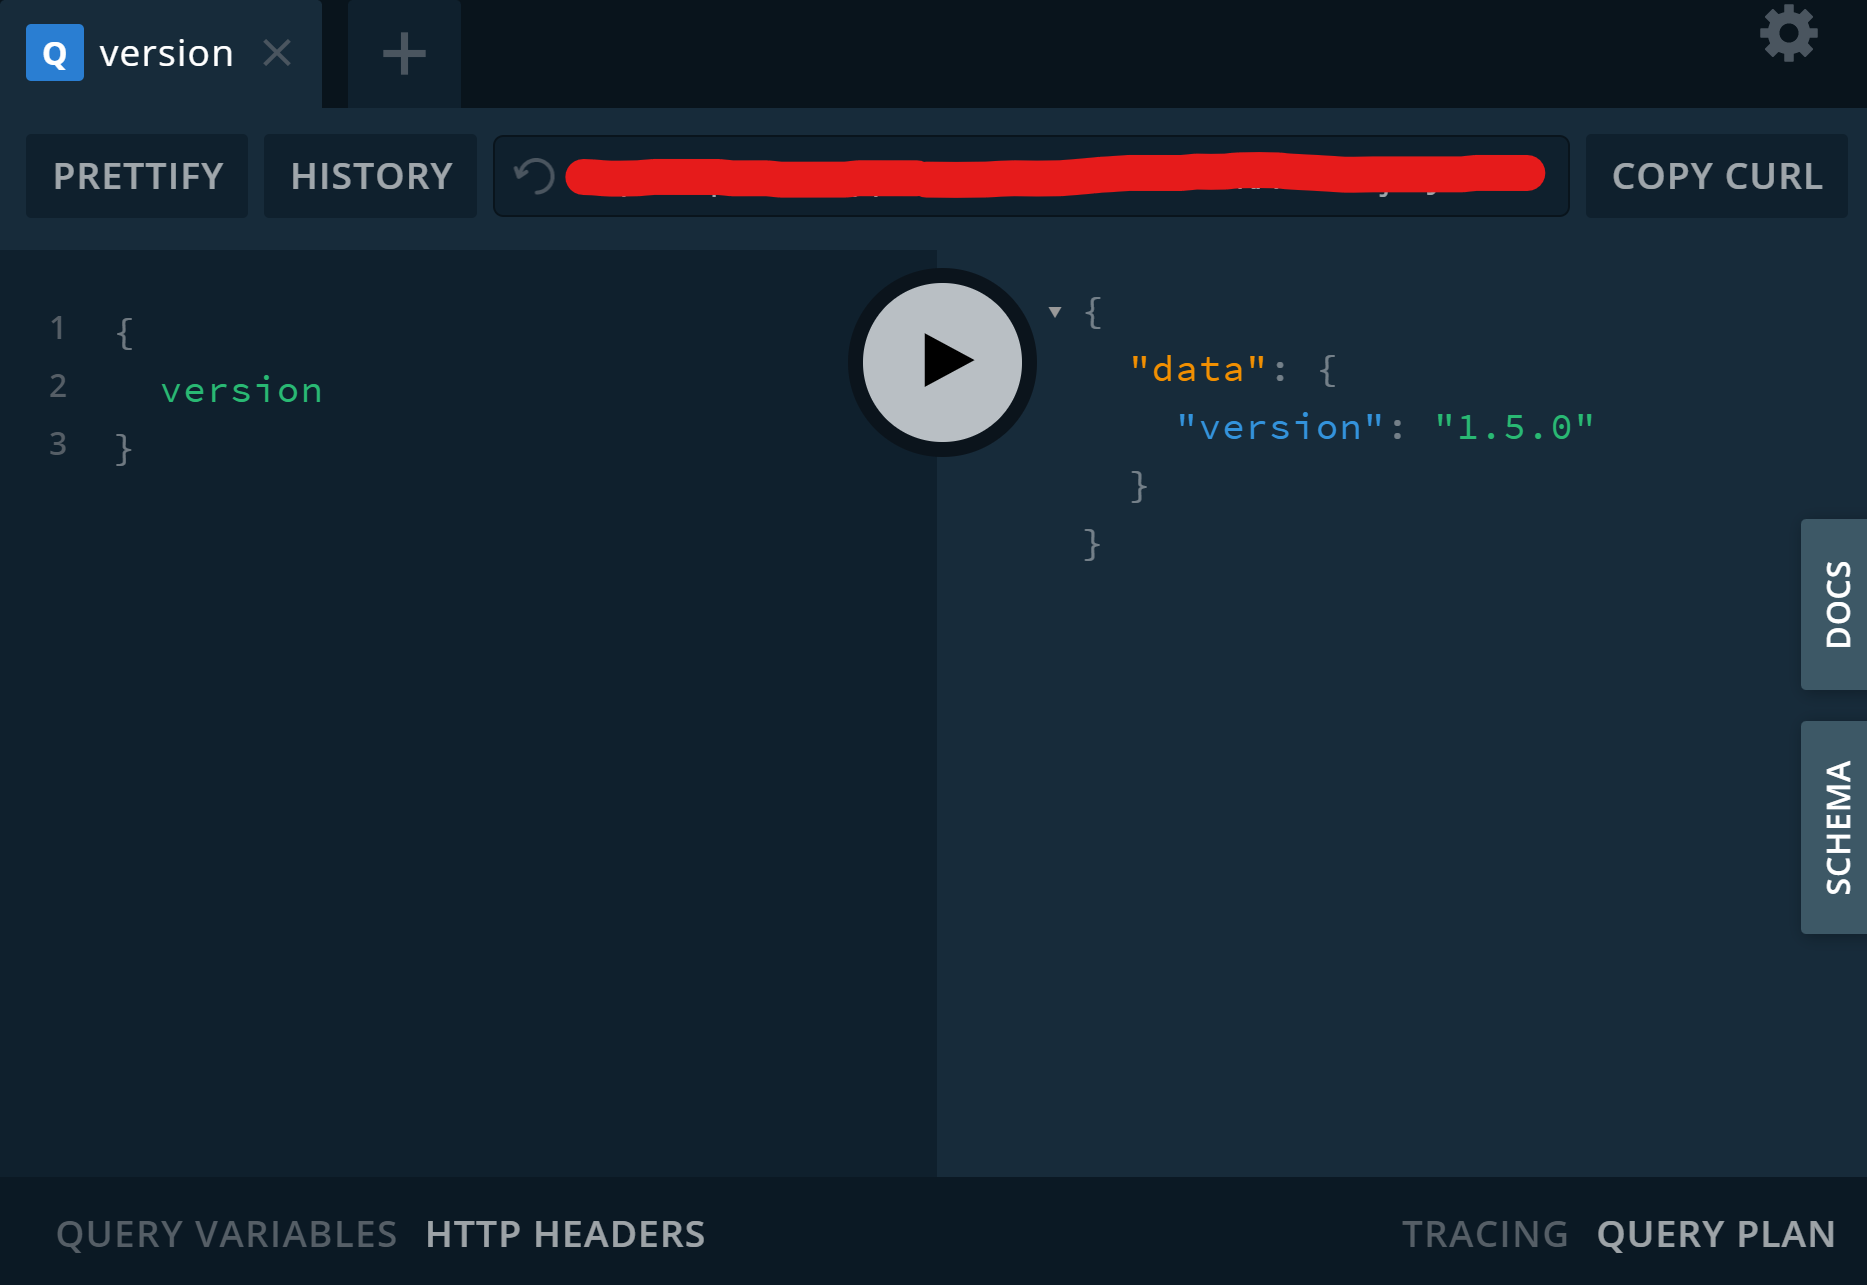
\includegraphics[scale=.35]{playground}
	\caption{محیط \lr{Playground} آپولو برای تست سرویس‌دهنده}
	\label{fig:playground}
\end{figure}
 

\section{درگاه ارتباط سریال}

پایگاه داده مونگو\footnote{\lr{MongoDB}}، یک نرم‌افزار پایگاه‌داده\footnote{\lr{Database}} متمرکز ولی توزیع‌پذیر، متن‌باز\footnote{\lr{Open Source}} و رایگان است که در دسته پایگاه‌های داده \lr{NoSQL} قرار می‌گیرد\cite{wiki:mongo}؛

در ابتدا لازم است بدانیم تفاوت این نوع پایگاه‌های داده با پایگاه‌های داده مرسوم \lr{SQL} چیست.

%\subsection{\lr{SQL}ها}

پایگاه‌های داده \lr{SQL} داده‌ها را در قالب جداولی نگهداری می‌کنند که هرکدام از آن‌ها دارای تعداد محدودی ستون، و تعداد نامحدودی ردیف هستند و در هر سلول این جداول، یک مقدار، خواه عددی باشد و خواه متنی و یا حتی اطلاعات خام\footnote{\lr{Raw}} بصورت دنباله‌ای از بایت\footnote{\lr{Byte}}‌ها، نگهداری می‌شود.

این جداول، نمی‌توانند بصورت افقی\footnote{\lr{Horizontal Scale}} رشد کنند و تنها حالت مقیاس‌پذیری آن‌ها از جهت عمودی\footnote{\lr{Vertical Scale}}، و با اضافه شدن ردیف‌های بیشتر به آن‌هاست. برای مثال اگر نیاز باشد تا خواص یک موجودیت\footnote{\lr{Entity}} که در این جدول‌ها با ستون‌ها نمایش داده می‌شوند را تغییر داد، تنها راه آن تغییر در طراحی کل جدول است و نمی‌توان برای ردیف‌های مختلف، خواص یا ستون‌های مختلف و یا حتی نامحدودی داشت.

همچنین گاهی اوقات، ساختار داده‌های ما به گونه‌ای است که بسیاری از موجودیت‌ها، شامل موجودیت‌های دیگری هستند؛ دراینصورت در \lr{SQL}ها باید این رابطه\footnote{\lr{Relation}}‌ها را با تعریف کلید‌های اولیه\footnote{\lr{Primary key}} و خارجی\footnote{\lr{Foreign Key}} تعریف کرد و اصطلاحا جداول را در حین اجرا با هم \lr{Join} کرد. اگر این ویژگی در ساختار موجودیت‌های ما بسیار زیاد و ملموس باشد، آن‌گاه اینگونه عملیات ممکن است بازدهی و کارآیی را بشدت کاهش دهد. در این شرایط، \lr{NoSQL}ها به کمک ما می‌آیند!\\

%\subsection{\lr{NoSQL}ها}

بطور کلی \lr{NoSQL}ها پایگاه‌های داده‌ای هستند که در آن‌ها ساختارهای موجودیت‌های بدون رابطه قابلیت تعریف شدن دارند و اکثرا در آن‌ها روش‌هایی برای رشد و مقیاس‌پذیری افقی داده‌ها پیش‌بینی شده است.

برای مثالی که در بخش قبلی مطرح شد، در یک پایگاه داده \lr{NoSQL} مانند مونگو براحتی می‌توان ساختار داده‌ای تعریف کرد که در آن مجموعه\footnote{\lr{Collection}}‌های موجودیت‌ها از لحاظ تعداد و یا حتی نوع ویژگی‌ها با هم متفاوت هستند اما در یک مجموعه نگهداری می‌شوند؛ درصورتی‌که موجودیت‌های تودرتو\footnote{\lr{Nested}} باشند، نیازی به ایجاد رابطه بین مجموعه‌های مختلف برای تکمیل آن‌ها نیست و به همان حالتی که در مجموعه خود ذخیره شده‌اند، موجودیت‌هایی که صریحا زیرمجموعه آن‌ها هستند بعنوان برخی از ویژگی‌های آن موجودیت ذخیره شده است و در واقع این ویژگی‌ها مانند ستون در جدول‌های \lr{SQL} هستند با این تفاوت که می‌توانند نامحدود و در طول مجموعه نابرابر و متفاوت باشند و همچنین مقادیر آن‌ها می‌تواند برخلاف \lr{SQL}، هر مقداری باشد، از مقادیر عددی و رشته‌ای تا ارایه\footnote{\lr{Array}} و یا حتی یک مجموعه کامل دیگر!\\

پایگاه‌های داده \lr{NoSQL} به 4 گروه تقسیم می‌شوند:
\begin{enumerate}
	\item کلید-مقدار\footnote{\lr{Key-Value}}: اطلاعات بصورت دوتایی کلید و مقدار ذخیره می‌شوند. مانند \lr{Redis}
	\item ستون عریض\footnote{\lr{Wide Column}}: دقیقا مشابه \lr{SQL}ها با این تفاوت که ستون‌های جداول می‌توانند متفاوت و یا نامحدود باشند. مانند \lr{Cassandra}
	\item سند محور\footnote{\lr{Document based}}: اطلاعات درقالب تعدادی فایل ساختاربندی شده با مقادیری مشابه ساختار \lr{JSON} نگهداری می‌شوند. مانند مونگو
	\item گراف محور\footnote{\lr{Graph based}}: اطلاعات در یال‌ها و گره‌های گراف نگهداری می‌شوند. مانند \lr{Neo4j}
\end{enumerate}

%\subsection{مونگو}
پس از بررسی انواع \lr{NoSQL}ها و تفاوت آن‌ها با \lr{SQL}ها، همانطور که گفتیم، مونگو (\cref{fig:mongo}) یکی از پایگاه‌های داده از نوع سند محور است و در دسته \lr{NoSQL}ها قرار می‌گیرد؛ با توجه به آمار اعلامی وبگاه \lr{DB-engine}، مونگو محبوب‌ترین پایگاه‌داده \lr{NoSQL} جهان است.\\

\begin{figure}[H]
	\centering
	
\includegraphics[scale=.3]{mongo}
	\caption{لوگوی مونگو}
	\label{fig:mongo}
\end{figure}

از ویژگی‌های منحصربفرد مونگو، می‌توان به موارد زیر اشاره کرد\cite{wiki:mongo}:
\begin{enumerate}
	\item تکثیر\footnote{\lr{Replica Set}}: با استفاده از قابلیت خودکار تکثیر مونگو، می‌توان مجموعه‌هایی از سرورهای مونگو ایجاد کرد که هرکدام یک کپی تکراری از داده‌ها را نگهداری می‌کنند؛ اما تمام آن‌ها می‌توانند جداگانه عمل خواندن اطلاعات و پرس‌وجو\footnote{\lr{Query}} را انجام دهند (البته فقط سرور اصلی می‌تواند عمل نوشتن و تغییر در داده‌ها را انجام دهد). همین ویژگی باعث افزایش بسیار زیاد سرعت و کارآیی می‌گردد.
	\item تعادل بار\footnote{\lr{Load Balancing}} و خوشه‌های خردشده\footnote{\lr{Sharded Clusters}}: با استفاده از این قابلیت، داده‌های مجموعه‌های مختلف به گونه‌ای خرد می‌شوند که هر مجموعه سرور، مسئول نگهداری بخشی از آن‌ها باشد و هر کدام از این بخش‌ها، توسط یک کلید خاص مشخص می‌شوند تا بتوانند بازیابی شده و بهم متصل شوند. 
	\item نگهداری و پرس‌وجو بهینه مختصات جغرافیایی: با استفاده از قابلیت فهرست‌سازی\footnote{\lr{Indexing}} از مختصات جغرافیایی و دستورات ویژه برای پرس‌وجوی آن‌ها که در نتیجه آن، استفاده از مونگو برای بسیاری از سیستم‌های مرتبط با مختصات جغرافیایی و یا سیستم‌های آب‌وهوایی بسیار بصرفه و بهینه شده است. همچنین مونگو قابلیت ایجاد فهرست از این مختصات‌ها را نیز داراست و این قابلیت سبب افزایش قابل توجه کارآیی و سرعت اجرای پرس‌وجوها برای یافتن نزدیک‌ترین مختصات به یک مختصات خاص، از درون مجموعه‌ی بسیار بزرگی از مختصات‌ها می‍شود، که در بسیاری از سیستم‌ها کاربرد فراوانی دارد.
	\item ذخیره فایل و تعادل بار آن: سیستمی تحت عنوان \lr{GridFS} که اجازه ذخیره فایل بعنوان داده در هر جایی از مجموعه‌ها را می‌دهد.
	\item خط لوله تجمیع\footnote{\lr{Aggregation Pipeline}}: مراحلی تحت عنوان مراحل خط لوله، که می‌توانند در یک فرآیند تجمیع، پشت سر هم اجرا شوند و خروجی‌ای از داده‌ها بسازند که در حالت عادی ممکن بود بسیار پیچیده و ساخت آن‌ها بسیار زمان‌بر باشد. همچنین این مراحل بطور خودکار توسط مونگو، اصلاح و بهینه می‌شوند؛ برای مثال بعضی از مراحل خط لوله مونگو، وقتی تحت شرایط خاصی، قبل یا بعد از یک مرحله خاص دیگر قرار می‌گیرند، می‌توانند حذف شوند و یا در مرحله دیگری ادغام شوند؛ مونگو به‌طور خودکار این ساده‌سازی را روی تمام دستورات خط لوله تجمیع انجام می‌دهد.
	\item پشتیبانی از ساختار رابطه‌ای: برخلاف اکثر پایگاه‌های داده \lr{NoSQL}، مونگو از ساختار رابطه‌ای نیز پشتیبانی می‌کند و معادلی نیز برای دستور \lr{Join} در \lr{SQL} دارد.
\end{enumerate}


\section{حسگر پالس‌اکسی‌متر}

ری‌اکت جی‌اس\footnote{\lr{ReactJS}} مجموعه‌ای از کتابخانه‌های جاواسکریپت برای تولید وب‌سایت و نرم‌افزارهای کاربردی تحت وب\footnote{\lr{Web application}} است که توسط فیسبوک\footnote{\lr{Facebook}} در سال 2013 توسعه داده شده و منتشر شده است. در واقع وقتی یک وب‌سایت با ری‌اکت (\cref{fig:react}) جی‌اس تولید می‌شود، علاوه بر ظاهر آن، منطق آن نیز در کنار ظاهر پیاده‌سازی می‌شود و با توجه به توسعه روزافزون نرم‌افزارهای کاربردی تحت وب تک صفحه‌ای\footnote{\lr{Single paged web applications}}، از ری‌اکت جی‌اس و رقبای آن (مانند انگولار\footnote{\lr{Google Angular}} و فلاتر گوگل\footnote{\lr{Google Flutter}} و ویوجی‌اس\footnote{\lr{VueJS}}) استقبال بسیاری شده است\cite{wiki:react}.

\begin{figure}[H]
	\centering
	
\includegraphics[scale=.1]{react}
	\caption{لوگوی ری‌اکت}
	\label{fig:react}
\end{figure}

%\subsection{آشنایی با ری‌اکت نیتیو}

ری‌اکت نیتیو\footnote{\lr{React Native}} بر پایه یکی دیگر از سرویس‌های محبوب فیس بوک یعنی ری‌اکت جی‌اس می‌باشد که در طراحی رابط کاربری استفاده می‌شود. ولی برخلاف ری‌اکت جی‌اس که تمرکز اصلی آن روی مرورگر است، ری‌اکت نیتیو برای ساخت اپلیکیشن‌های موبایل استفاده می‌شود\cite{wiki:react}.
درواقع  ری‌اکت نیتیو یک چارچوب توسعه اپلیکیشن های چند سکویی است (که جلوتر توضیح داده خواهند شد).

برنامه‌های ری‌اکت نیتیو با زبان جاواسکریپت و \lr{JSX} نوشته می‌شوند. سپس می‌توان از این کدها برای اندروید و \lr{iOS} خروجی گرفت.\\

نرم افزارهای کاربردی متناسب با پلتفرمی که روی آن‌ها اجرا خواهند شد به دو دسته تقسیم می‌شوند:
\begin{enumerate}
	\item اپلیکیشن بومی یا نیتیو\footnote{\lr{Native}}
	\item اپلیکیشن چندسکویی یا \lr{Cross Platform}
\end{enumerate}


%\subsection{اپلیکیشن بومی}

به اپلیکیشن‌هایی گفته می‌شود که برای یک پلتفرم خاص توسعه داده شده‌اند. وقتی شما می‌خواهید یک اپلیکیشن نیتیو بسازید باید از زبان اصلی که برای آن پلتفرم پیشنهاد شده است استفاده کنید. برای مثال برای نوشتن یک اپلیکیشن نیتیو اندروید\footnote{\lr{Android}} باید از زبان کاتلین\footnote{\lr{Kotlin}} (از جاوا هم برای نوشتن اپلیکیشن‌های نیتیو اندروید می‌توان استفاده کرد) استفاده کنید. وقتی از کاتلین استفاده می‌کنید اپلیکیشن شما به صورت نیتیو (بومی) فقط روی سیستم عامل اندروید اجرا خواهد شد.

%\subsection{اپلیکیشن چندسکویی}

به اپلیکیشن‌هایی گفته می‌شود که برای چند پلتفرم توسعه داده می‌شوند.
در این حالت با استفاده از یک سری فریم ورک ها میتوان اپلیکیشنی توسعه داد که برای همه ی پلتفرم‌ها قابل نصب و اجرا باشد.
در واقع با استفاده از یک کد قادر خواهید بود تا برای پلتفرم‌های اندروید، \lr{iOS}، وب و ... خروجی قابل استفاده بگیرید.
آمار استفاده از این نوع چارچوب‌ها در \cref{fig:rnstat} قابل مشاهده است.

\begin{figure}[h!]
	\centering
	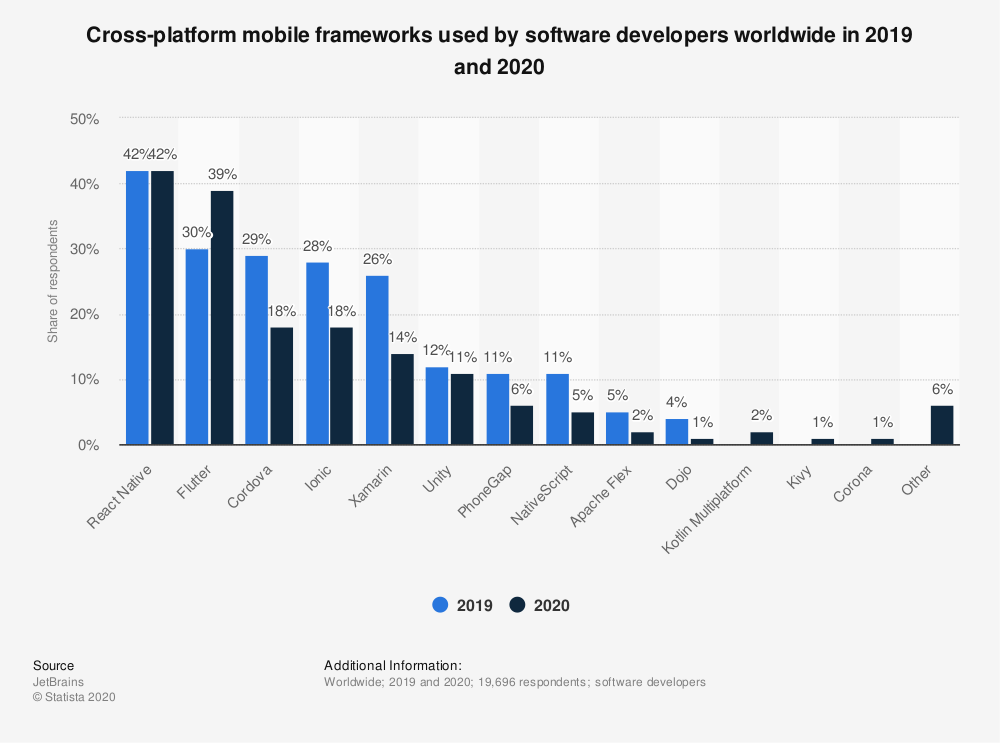
\includegraphics[scale=0.45]{rnstat.png}
	\caption{آمار استفاده فریم‌ورک‌های چندسکویی جهان در سال 2019\cite{react:crossplatform}}
	\label{fig:rnstat}
\end{figure}


%\subsection{ساختار کلی برنامه‌های ری‌اکت نیتیو}

از یک دیدگاه سطح بالا به رابط کاربری برنامه‌های تلفن همراه، هر برنامه از تعدادی صفحه تشکیل می‌شود که کاربران در تعامل با عناصر موجود در رابط کاربری، بین این صفحات جابجا می‌شوند‌\cite{wiki:react}.

رابط کاربری گرافیکی در ری‌اکت نیتیو به زبان \lr{JSX} نوشته می‌شود. عناصر رابط کاربری، کامپوننت\footnote{\lr{Component}} نامیده می‌شوند. به عنوان مثال عکس‌ها، متن‌ها و دکمه‌ها، کامپوننت‌هایی هستند که به صورت از پیش تعریف شده در ری‌اکت نیتیو وجود دارند. برنامه‌نویس از کنار هم گذاشتن این عناصر و چینش آن‌ها در یک صفحه، رابط کاربری را طراحی می‌کند. همچنین کامپوننت‌های دلخواه نیز می‌تواند توسط برنامه‌نویس ایجاد گردد.

پیاده‌سازی منطق برنامه، یعنی اتصال به سرور، مدیریت داده‌ها، گرفتن ورودی‌های کاربر و پردازش آن‌ها با زبان جاوا اسکریپت پیاده‌سازی می‌گردد.



مانند هر نرم‌افزار دیگری، برنامه‌های تلفن همراه توسعه داده‌شده با ری‌اکت نیتیو، با اطلاعات کاربران سر و کار دارد. در ری‌اکت نیتیو روش‌های متعددی برای ذخیره و مدیریت داده‌ها تعبیه شده است که هر کدام از آن‌ها برحسب نیاز به کار می‌رود. روش‌ها به طور خلاصه به شرح زیر می‌باشند\cite{wiki:react}:
\begin{itemize}
	\item متغیر\footnote{\lr{Variable}}های معمولی جاوا اسکریپت: این نوع متغیرها برای ذخیره‌ی داده‌های میانی و موقت به کار می‌روند و نقش چرک‌نویس را دارد.
	\item متغیرهای ثابت\footnote{\lr{Constant}} جاوا اسکریپت
	\item \lr{Props}: یک کامپوننت برای نمایش‌اش ممکن است نیاز به یک سری داده‌ها داشته باشد. این داده‌ها به صورت متغیرهایی به نام \lr{props} از کامپوننت بیرونی به آن‌ها منتقل می‌شوند. همانند نوع \lr{constant}، این متغیرها ثابت هستند.
	\item \lr{State}: از این نوع متغیرها برای ذخیره‌ی اطلاعات مربوط به کامپوننت استفاده می‌شود. به عنوان مثال، برای ذخیره‌ی متن نوشته شده توسط کاربرد در یک فیلد متنی، برای ذخیره‌ی وضعیت یک دکمه و... . این نوع متغیرها قابل تغییر می‌باشند.
	\item \lr{Context}: اگر بخواهیم داده‌ای را چندین لایه به کامپوننت های درونی‌تر پاس بدهیم، یک راه این است به کمک \lr{props}ها مرحله به مرحله متغیر را به کامپوننت درونی‌تر پاس بدهیم تا سر انجام به درونی‌ترین آن‌ها برسد. اما چنین کاری، مطمئنا بهینه نمی‌باشد. راهکار بهتری که در ری‌اکت نیتیو تعبیه شده این است که چنین داده‌هایی، در یک فضای گلوبال تحت عنوان \lr{context} تعریف می‌شوند و به کامپوننت هایی که می‌خواهیم به این داده‌های دسترسی داشته باشند، اجازه‌ی دسترسی می‌دهیم.\newline
\end{itemize}

\section{حسگر شتاب خطی و سرعت زاویه‌ای}

\section{صفحه نمایش}

\section{مدار شارژ و مدیریت توان}

\section{موتور ایجاد لرزش}

\section{بازر}

\section{کلیدهای لمسی}